\documentclass[12pt,a4paper,UTF8]{article}
\usepackage{ctex} % Chinese support
\usepackage{graphicx} % Insert images
\usepackage{listings} % Print source code
\usepackage{color} % Color support
\usepackage{booktabs} % Professional table support
\usepackage{pdflscape} % Landscape pages support in PDF
\usepackage{hyperref} % Hypertext links support for cross-referencing

% Customize hyperref format (it's set to no special format here)
\hypersetup{hidelinks}

% Declare directories to search for graphics files for graphicx
\graphicspath{{figures/}{logo/}}

% Define source code style for listings
\lstdefinestyle{c}{
  language=C,
  basicstyle=\ttfamily\footnotesize,
  keywordstyle=\bfseries\color[rgb]{0, 0, 1},
  identifierstyle=\color[rgb]{0.5, 0.3, 0.1},
  stringstyle=\color[rgb]{0.6, 0.1, 0.1},
  commentstyle=\itshape\color[rgb]{0.05, 0.5, 0.05},
  backgroundcolor=\color[gray]{0.95},
  numbers=left,
  numbersep=5pt,
  numberstyle=\color[gray]{0.6},
  breaklines=true
}
\lstdefinestyle{asm}{
	language=python,
	basicstyle=\ttfamily\footnotesize,
	keywordstyle=\bfseries\color[rgb]{0, 0, 1},
	identifierstyle=\color[rgb]{0.5, 0.3, 0.1},
	stringstyle=\color[rgb]{0.6, 0.1, 0.1},
	commentstyle=\itshape\color[rgb]{0.05, 0.5, 0.05},
	backgroundcolor=\color[gray]{0.95},
	numbers=left,
	numbersep=5pt,
	numberstyle=\color[gray]{0.6},
	breaklines=true
}

% Define new command for title page
\newcommand{\reporttitle}[2]{
  \LARGE\textsf{#1}\quad\underline{\makebox[12em]{#2}}
}
\newcommand{\reportinfo}[2]{
  \large\makebox[4em]{\textsf{#1}}\quad\underline{\makebox[18em]{#2}}
}

% The document begins here
\begin{document}
\begin{titlepage}
  \centering
  \vspace*{\fill}
  
\includegraphics[height=144pt]{nju-logo}\\[48pt]
  {\huge\textsf{课\ 程\ 实\ 验\ 报\ 告}}\\[48pt]
  \reporttitle{实验名称}{简单引导程序的实现}\\[72pt]

  \reportinfo{课程名称}{操作系统}\\[8pt]
  \reportinfo{院\hspace{\fill}系}{计算机科学与技术系}\\[8pt]
  \reportinfo{学\hspace{\fill}号}{191220129}\\[8pt]
  \reportinfo{姓\hspace{\fill}名}{邢尚禹}\\[8pt]
  \reportinfo{邮\hspace{\fill}箱}{191220129@smail.nju.edu.cn}\\[8pt]
  \reportinfo{实验日期}{2021年3月}\\
  \vspace*{\fill}
\end{titlepage}

\tableofcontents
\newpage
\section{实验进度}
已完成所有内容。

\section{实验过程及结果}
\subsection{在实模式下打印hello world}
查阅相关资料知,通过int 0x10可以打印字符串,其中(dl, dh)为坐标,al, bl为属性,bx为页码,cx为长度,ah为0x13,bp为字符串地址。据此写汇编代码如下:
\lstinputlisting[style=asm]{real.s}
运行结果:
\begin{figure}[htbp]
	\centering
	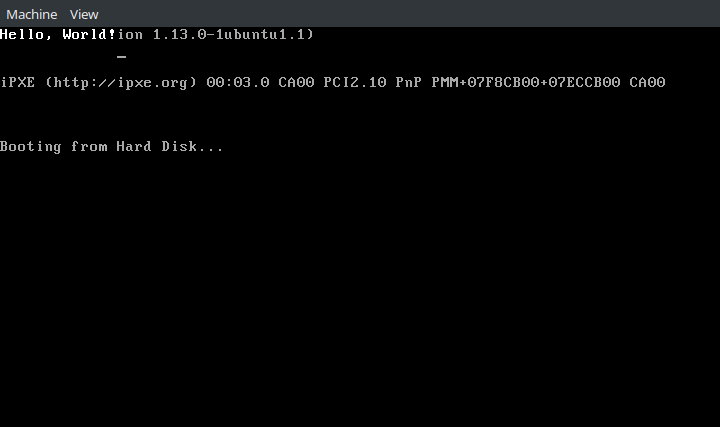
\includegraphics[width=\textwidth]{real}
	\caption{实模式下的运行结果}
\end{figure}

\subsection{在保护模式下打印hello world}
\subsubsection{从实模式到保护模式的切换}
关闭中断,打开A20数据总线,加载 GDTR ,设置 CR0 的PE位(第0位)为 1 ,通过长跳转设置 CS 进入保护模式。
\lstinputlisting[style=asm]{r2p.s}
\subsubsection{在保护模式中打印hello world}
只需要把字符串(带字符属性信息)写入显存0xb8000处即可。为输出白色字符,可将属性信息设置为字节0x0f。
\lstinputlisting[style=asm]{print.s}
\begin{figure}[htbp]
	\centering
	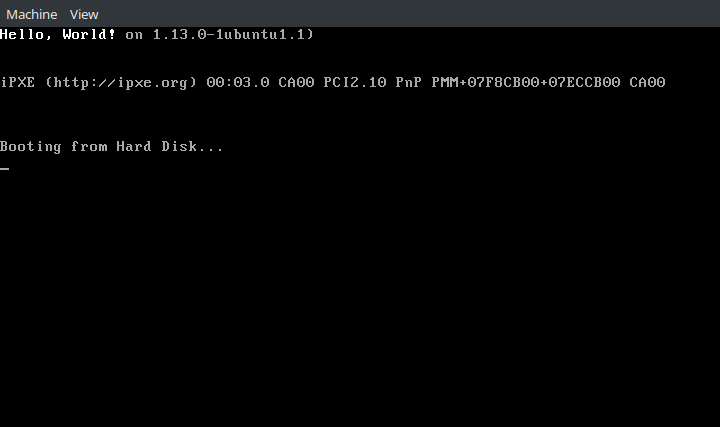
\includegraphics[width=\textwidth]{protected}
	\caption{保护模式下的运行结果}
\end{figure}

\newpage
\subsection{在保护模式下装载程序}
调用readSect函数装载程序,再跳转执行即可。
\lstinputlisting[style=c]{load.c}
测试结果:
\begin{figure}[htbp]
	\centering
	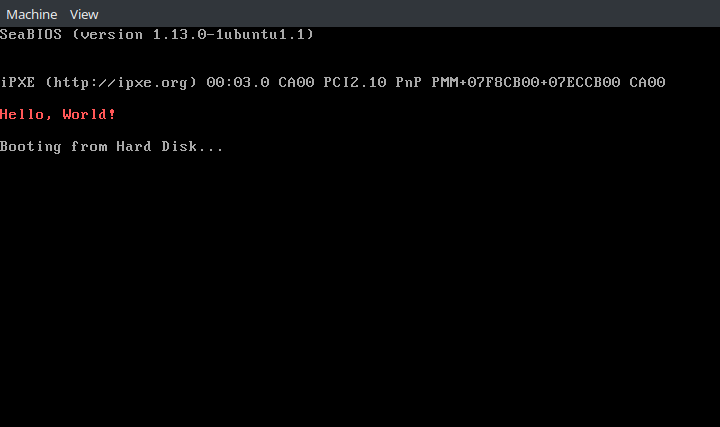
\includegraphics[width=\textwidth]{load}
	\caption{程序装载的运行结果}
\end{figure}

\section{困难与建议}
实验指导文档总体设计不太合理。例如,从实模式到保护模式的切换部分,大量篇幅在介绍GDTR等内容,但这些已经在ics课上学过,没有太大必要;但是A20数据总线的内容并没有详细介绍,需要自己查阅资料,比较耗费时间。
另外,建议增加一些对汇编语言的介绍,例如如何定义字符串,如何设置全局变量等。.word,.byte这些内容都没有学过,加一些简单介绍会更好。

\end{document}